\documentclass{article}
\usepackage[utf8]{inputenc}

\usepackage[english]{babel}

\usepackage[colorlinks=true, allcolors=blue]{hyperref}

\usepackage{graphicx}

\usepackage{natbib}
\bibliographystyle{unsrtnat}

\usepackage{amsmath}

\begin{document}

We implement the backward-forward Monte-Carlo method (BFMT) described in details in \cite{yong2016}.
The idea is to propagate a certain number of unpolarized light rays backward (i.e. from the instrument) and see where they end up.
The radiant flux of the ground at the end point is associated to the ray.
Once the ray touches the ground, we can trace it forward from the ground to the instrument to compute its polarisation at each scattering event.
Then we can just add all rays together to get the polarisation due to multiple scattering.\\

This has the huge advantage over forward monte carlo simulation to reduce th number of useless rays drastically, as all computed rays reach the detector. However, we still have to disregard the rays escaping toward space, and the rays touching ground too far from the instrument where we do not have any emmision data.\\

\section{Backward propagation}

An unpolarised ray of undefined intensity is propagated from the instrument detector along its line of sight.
At every predifined step of length $l$, the rays has a given probability to be scattered.
This probability is defined at every altitude as the scattering cross-section of the air and aerosols.
From \cite{bucholtz1995}, we have the Rayleigh scaterring cross-section per volume of atmosphere:
\begin{equation}
\beta(\lambda, z) = \beta_0(\lambda) \frac{P(z)}{P_0} \frac{T_0}{T(z)}\,,
  \label{eq:beta_z}
\end{equation}
with $P(z)$ and $T(z)$ the atmospheric pressure and temperature profiles.
$P_0 = 101\,325$ Pa and $T_0 = 288.15$ K are the pressure and temperature at sea level, and
\begin{linenomath*}\begin{equation}
    \beta_0(\lambda) = A_{ray}\lambda^{-(B+C\lambda + D/\lambda)}\,,
    \label{eqn:sqlaw}
\end{equation}\end{linenomath*}
with $\lambda$ the wavelength (in $\mu$m).

We also have the aerosol cross-section $C_{aer}$.

For now, I take as the probability of scattering for the ray:
\begin{equation}
  p(sca) = (\beta + C_{aer}) l
\end{equation}


The scattering angle is choosen at random using the scattering phase function for Rayleigh and Mie scattering.
The probability of a scattering angle $\theta$ is given by:
\begin{equation}
  p(\theta) = \frac{\beta \Phi_{ray}(\theta) + C_{aer} \Phi_{aer}(\theta)}{\beta + C_{aer}}
\end{equation}

The scattering plane is also random and unique for each ray. All scattering events of a single ray will take place in the same scattering plane. We use a uniform distribution of scattering planes.

The following figures illustrate the path computation of the rays for an instrument pointing northward at 45 degrees elevation. 1000 rays were computed in 2 min on my 4 laptop processors. This time can certainly be greatly improved easely by being a bit more clever.

\begin{figure}
  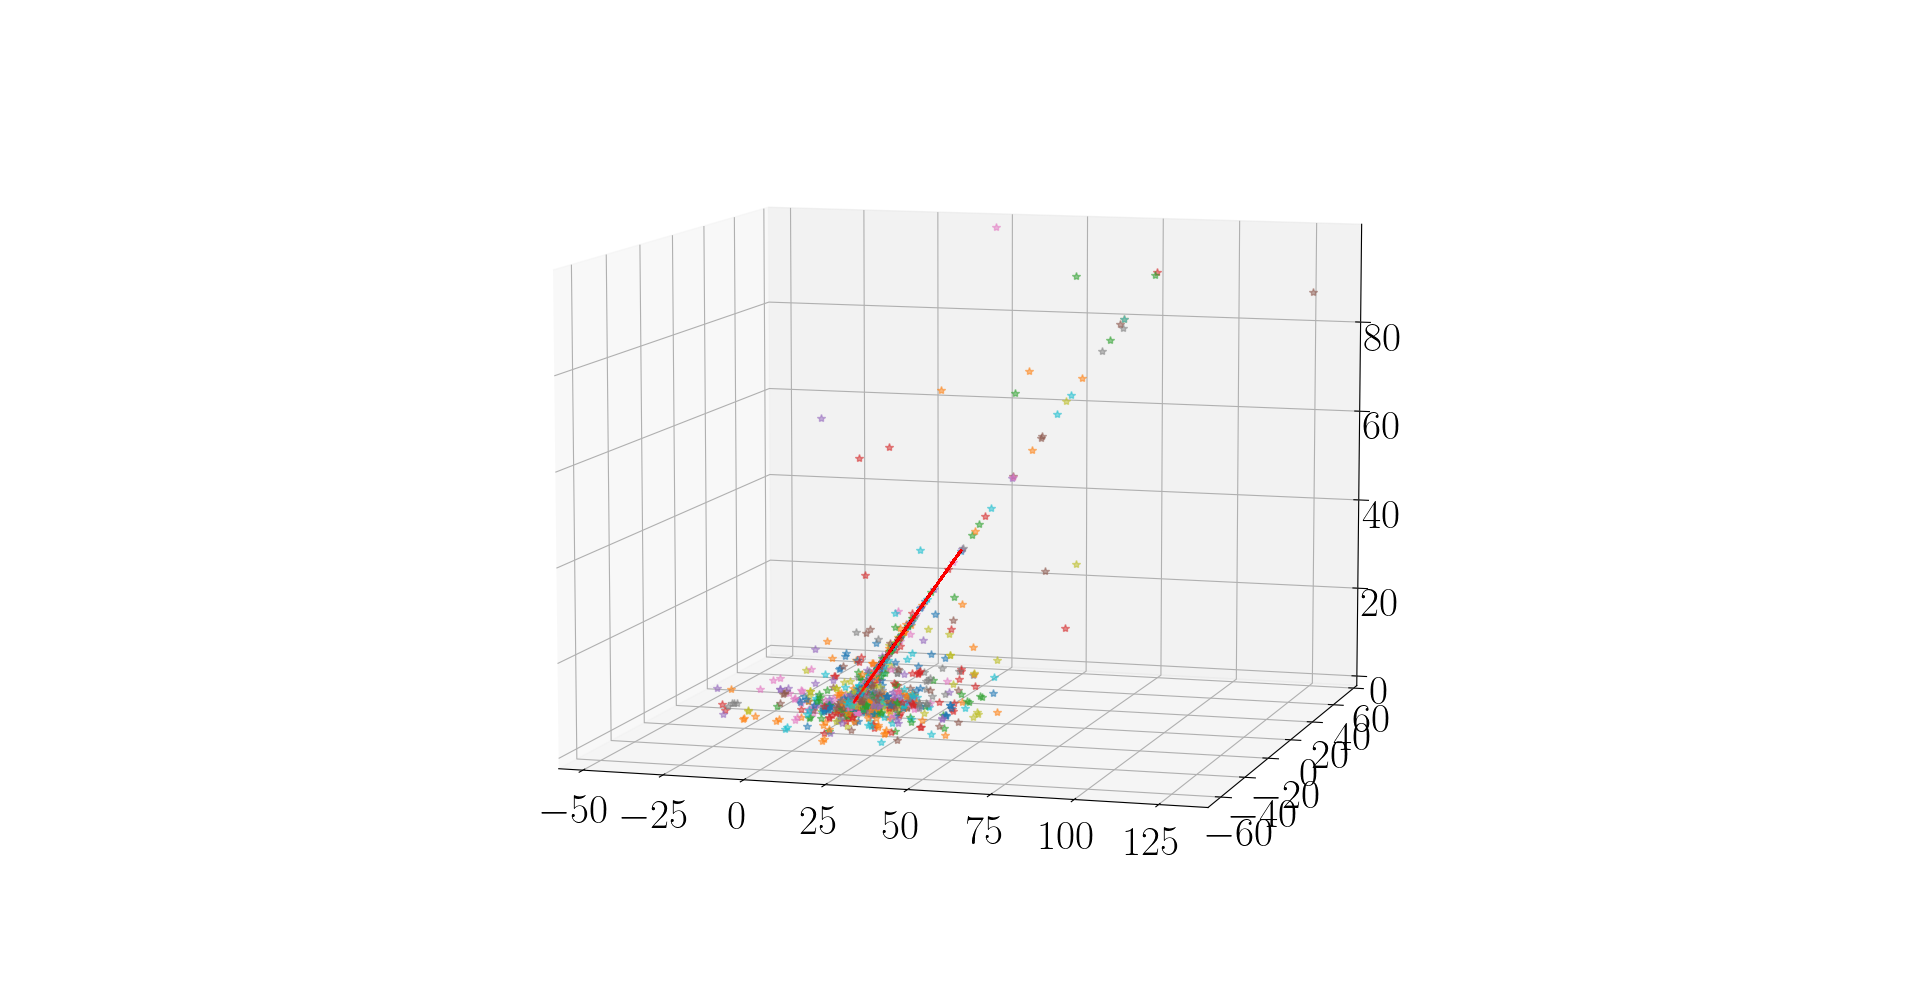
\includegraphics[width=\textwidth]{MS_3D_events.png}
  \caption{3D plots of all scattering events of a 1000 scattered rays. The line of sight of the instrument (red line) is clearly visible just with the points.}
\end{figure}

\begin{figure}
  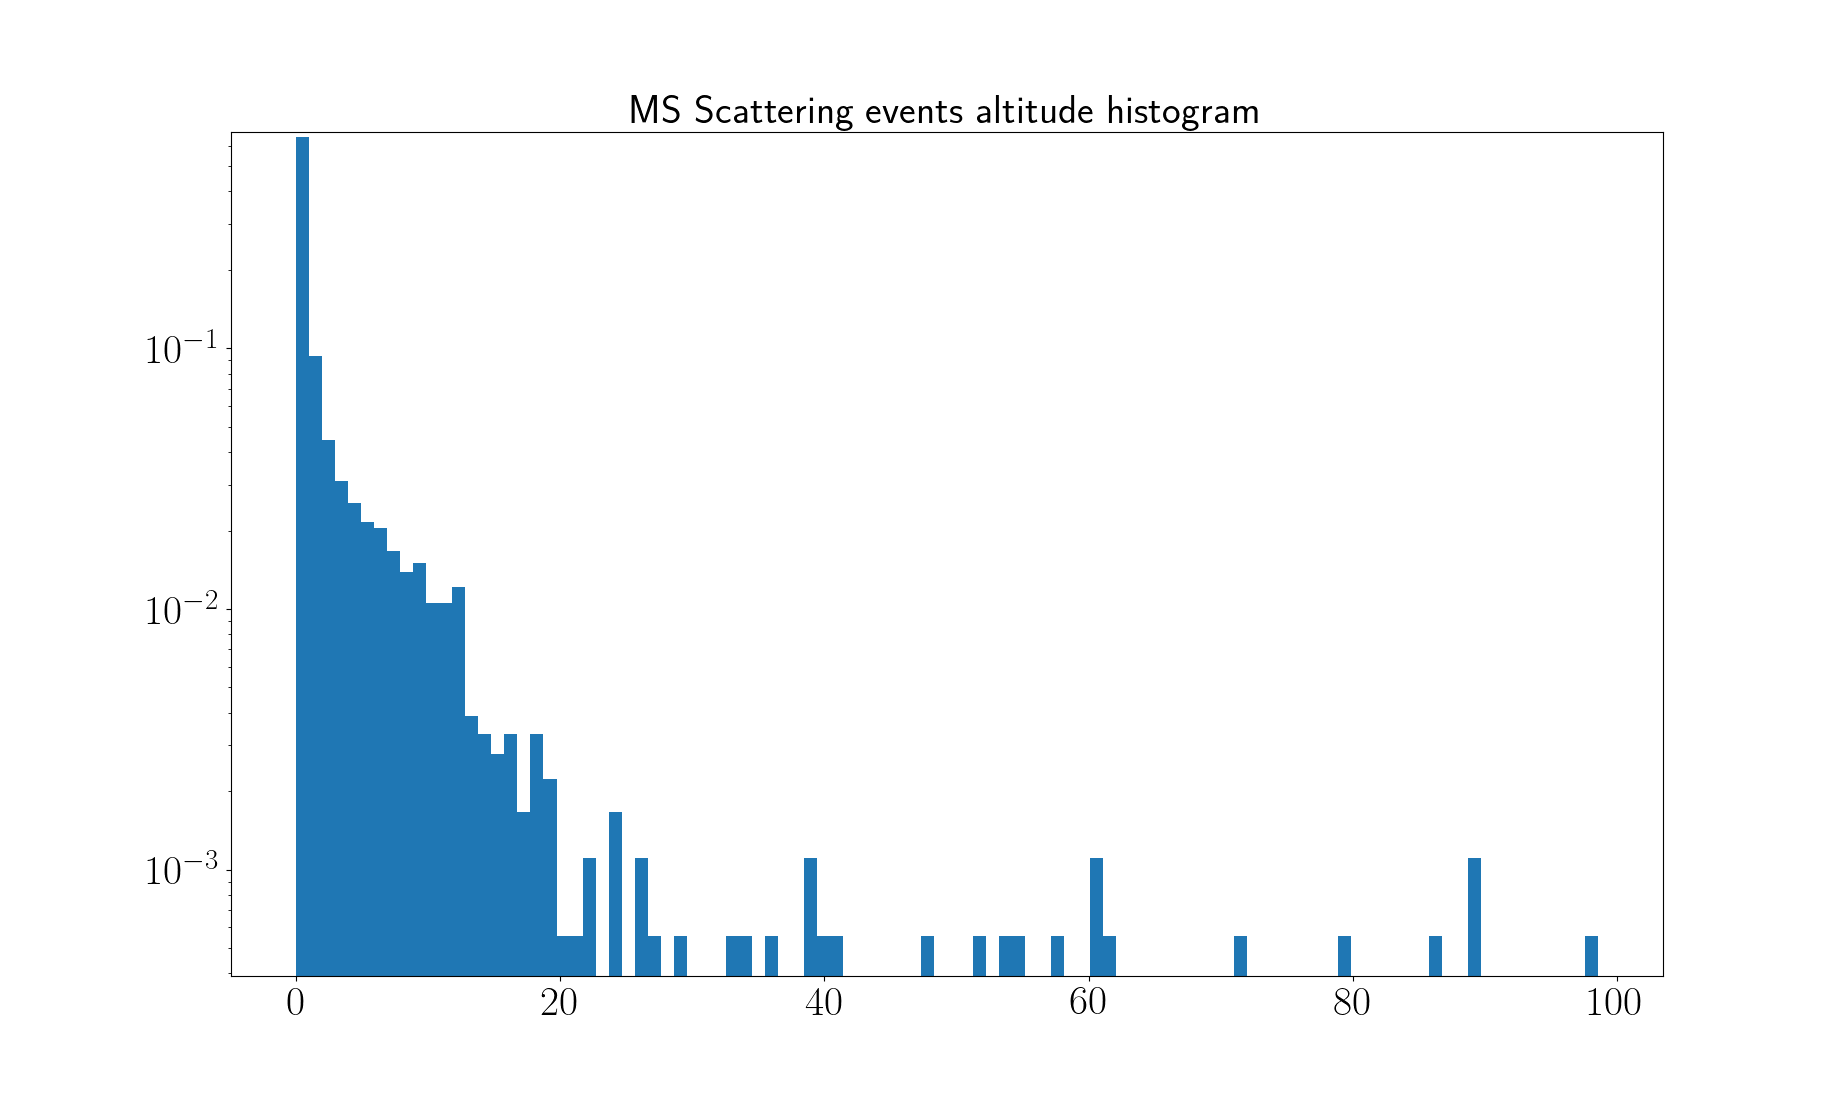
\includegraphics[width=\textwidth]{MS_alt_histo.png}
  \caption{Histogram of the scattering altitudes of scattering events for 1000 rays.}
\end{figure}
\begin{figure}
  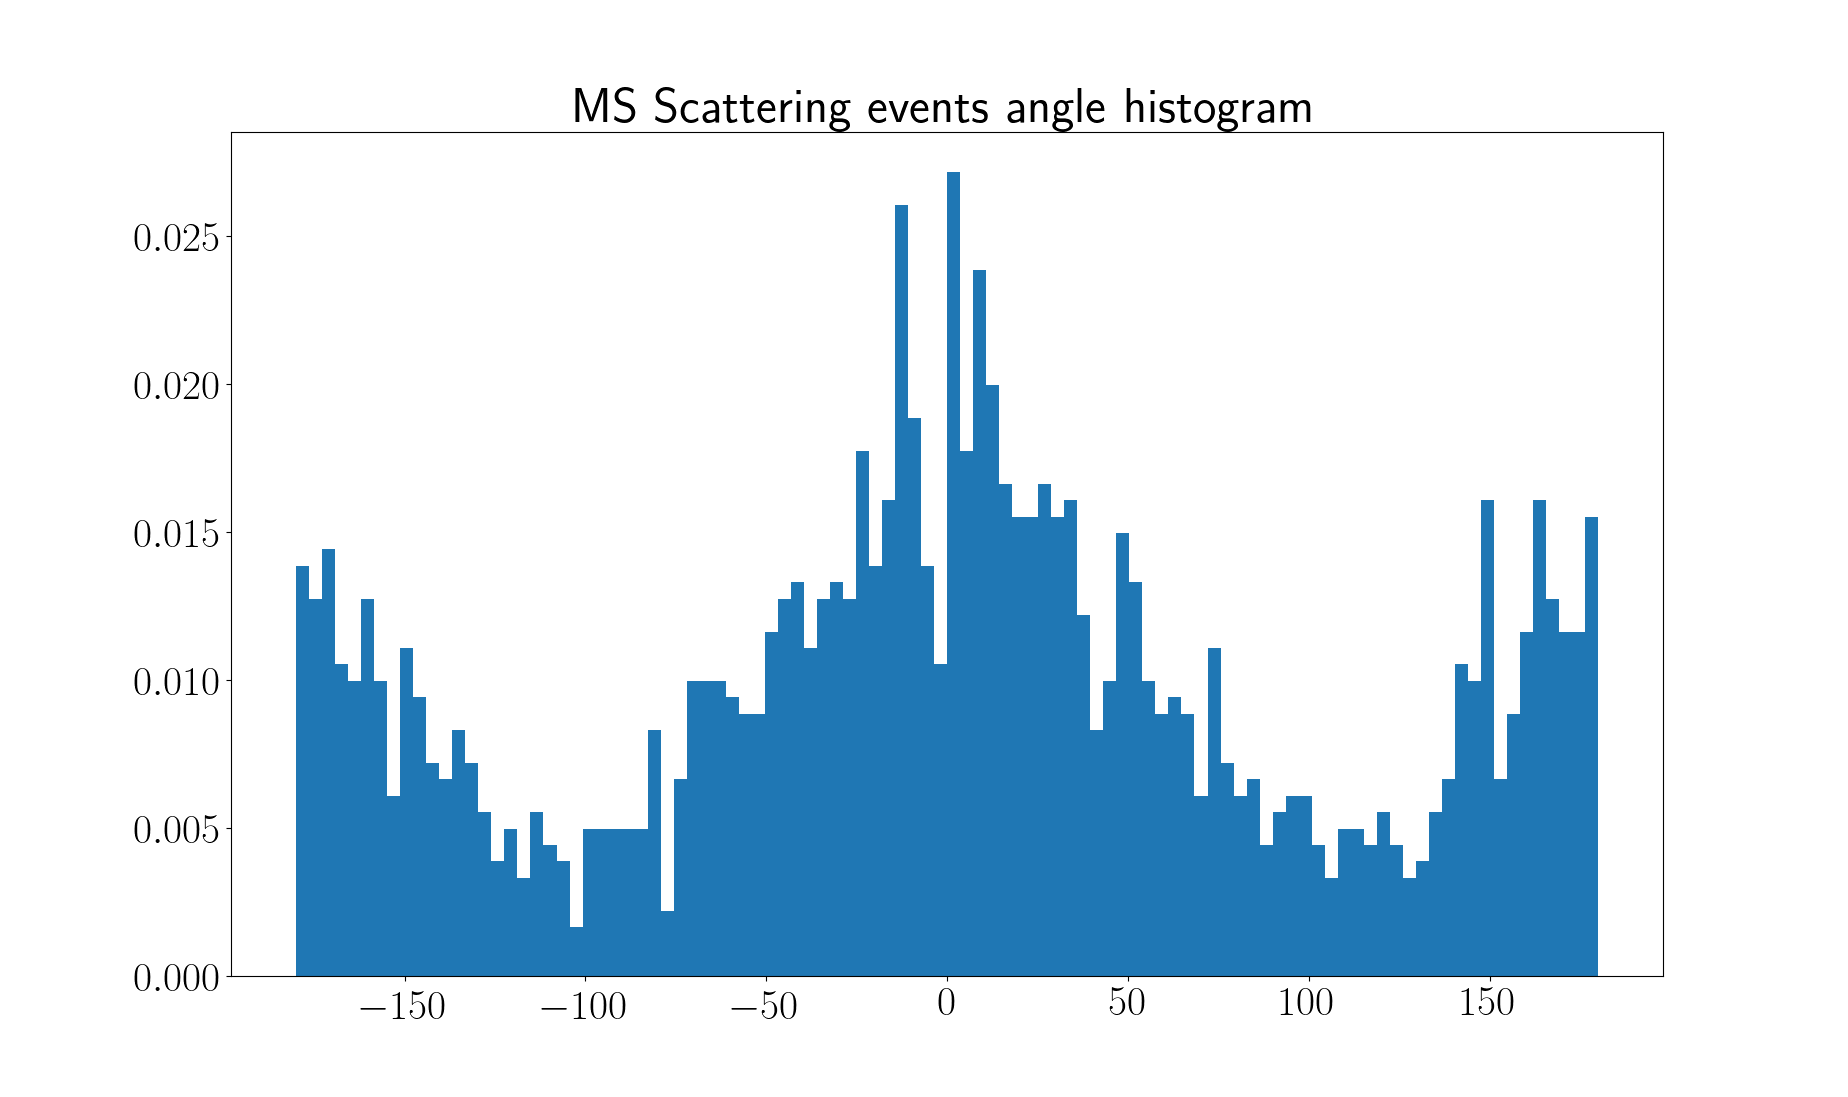
\includegraphics[width=\textwidth]{MS_sca_angle_histo.png}
  \caption{Histogram of the scattering angle of all scattering events for 1000 rays.}
\end{figure}

\begin{figure}
  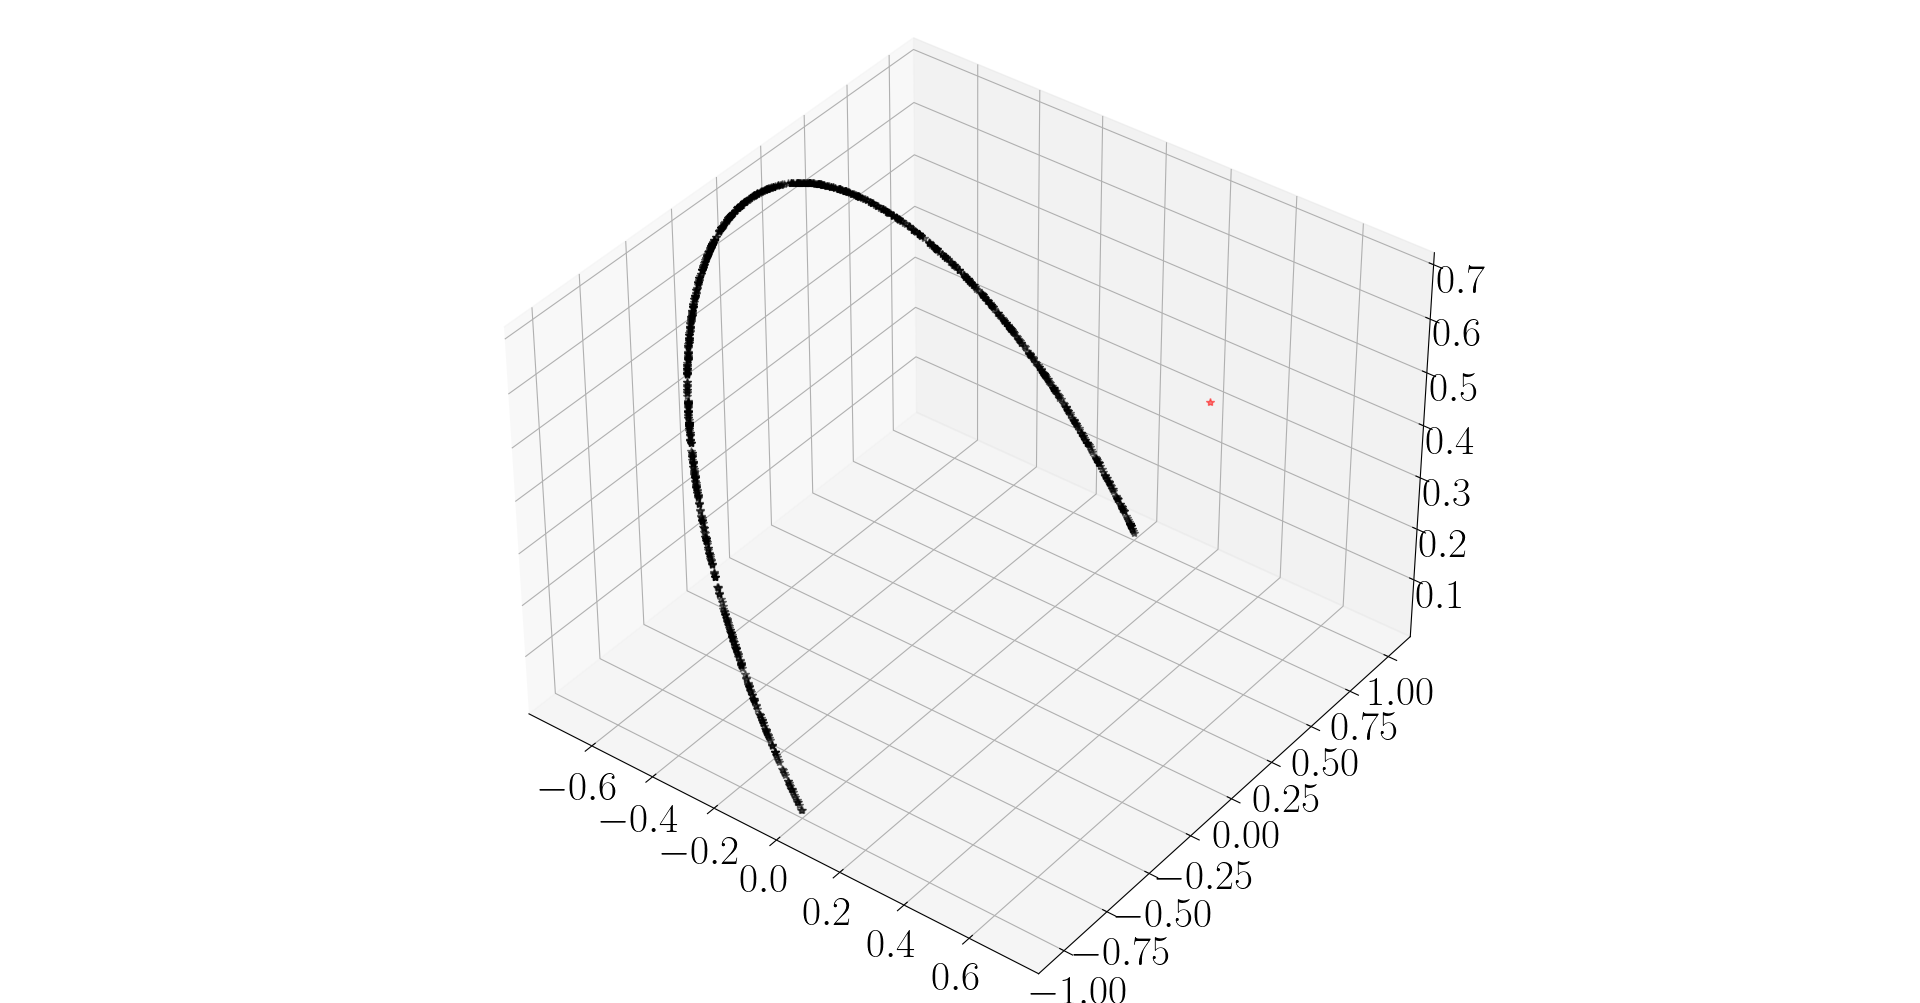
\includegraphics[width=\textwidth]{MS_sca_plane.png}
  \caption{Distribution of the scattering planes for a 1000 rays. Red dot is the line of sight of the instrument (elevation 45$^\circ$). Black dots are the normal vectors of the 1000 scattering planes. The distribution is uniform across all angles.}
\end{figure}

\begin{figure}
  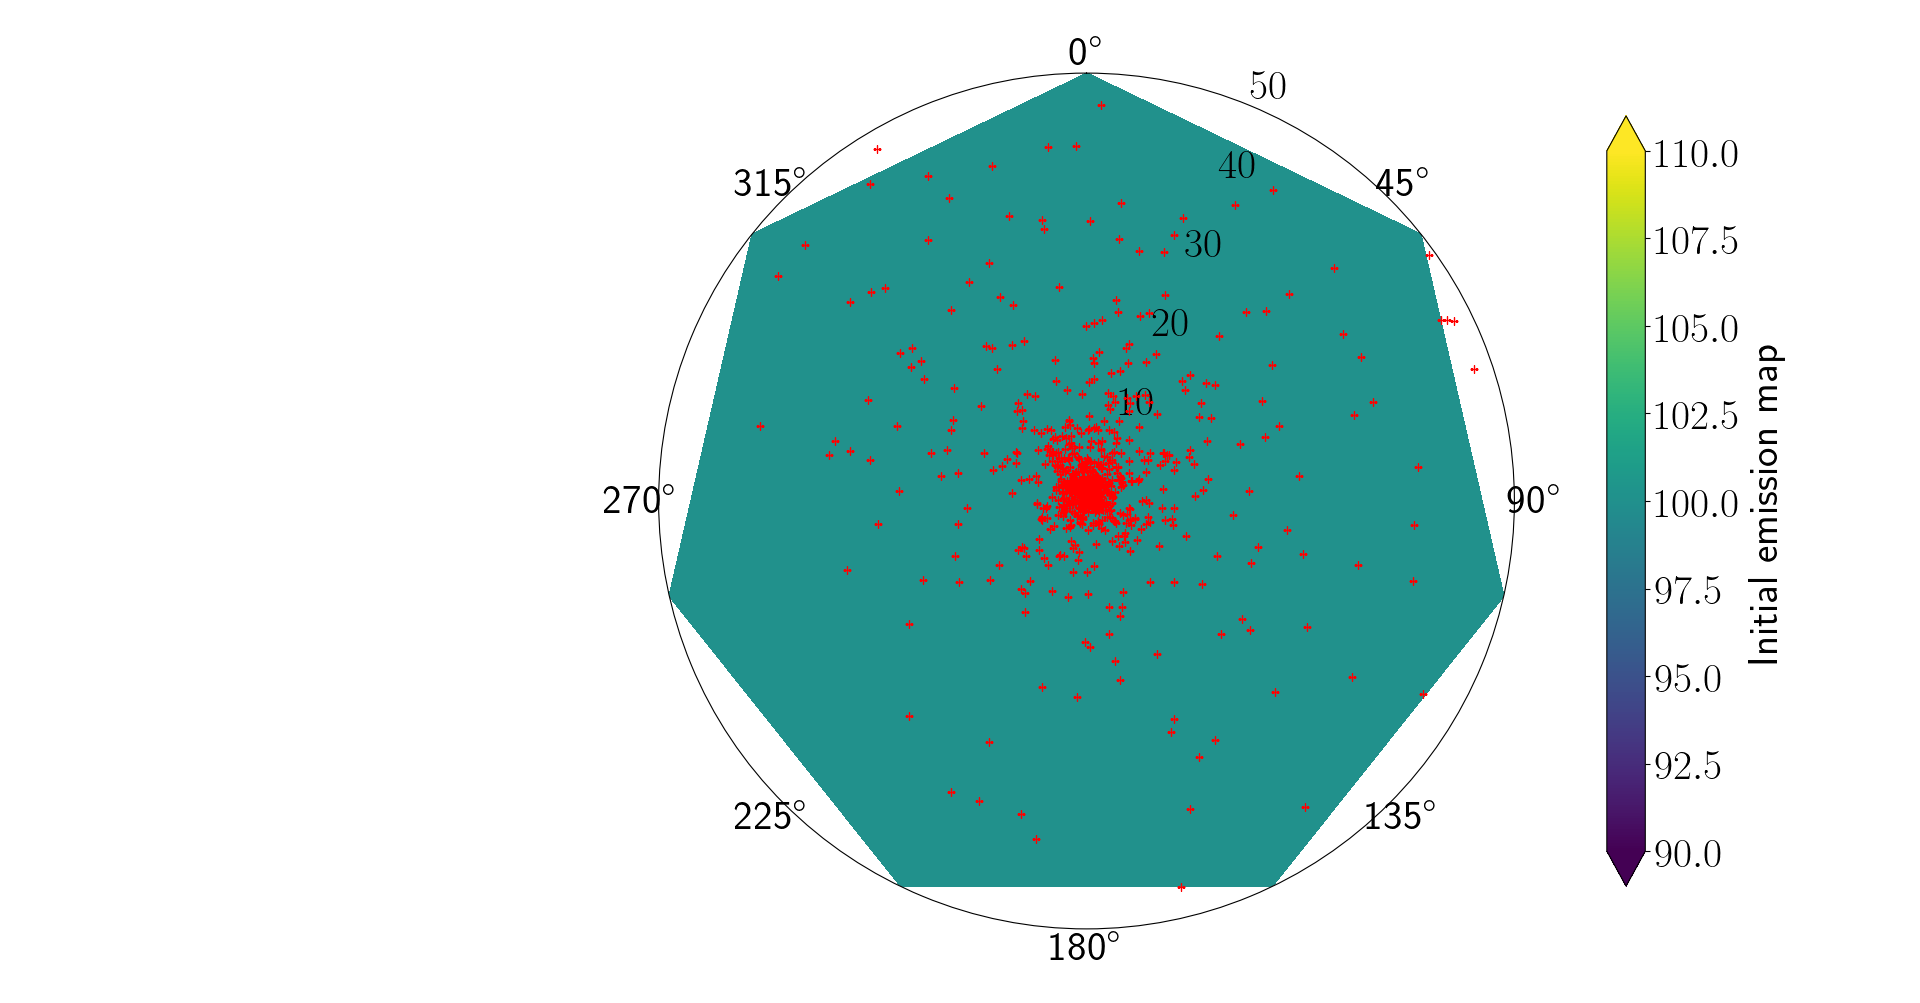
\includegraphics[width=\textwidth]{MS_uniform_grd_endpoints.png}
  \caption{Uniform ground emission map used as an example. Red cross are the end points of 1000 rays, i.e. the position where the ray intersect the ground.}
\end{figure}



\section{Forward propagation}

Once a ray has touch the ground somwhere near the instrument, we can trace it back to the detector and compute its polarisation after each scattering event.

We assume the ray is unpolarised at the emission, with Stokes vector ($I = 1$, $Q = 0$). They are defined with respect to the scattering plane of the ray, such that $Q=1$ correspond to a perpendicular polarisation and $Q=-1$ a plane-parallel  polarisation.
We assume that Rayleigh and Mie scattering only affect $Q$, and not $U$, so that we do not compute $U$ at this point. We also do not compute circular polarisation and omit the fourth Stockes paramter $V$.

For each scattering event of the ray from the ground toward the instrument, the Stockes vector is updated with the corresponding scatteing matrix $M$.
The scattering matrix for Rayleigh and Mie scattering ($M_{ray}, M_{aer}$) are computed and merged to give the scattering matrix at a given altitude $z$:
\begin{equation}
  M = \frac{\beta(z) M_{ray} + C_{aer}(z) M_{aer}}{\beta + C_{aer}}
\end{equation}

For Rayleigh scattering,
\begin{equation}
M_{ray} = \frac{3}{4}
\begin{pmatrix}
\cos^2(\theta) + 1 & \cos^2(\theta) - 1\\
\cos^2(\theta) - 1 & \cos^2(\theta) + 1

\end{pmatrix}
\end{equation}

POUR CETTE MATRICE DE DIFFUSION, JE NE SUIS VRAIMENT PAS SUR DE MOI ET J'AI PRIS QUELQUE CHOSE DE PLAUSIBLE POUR FAIRE TOUNER LE CODE. MAIS IL Y A DES CHANCES QUE CE NE SOIT PAS JUSTE !
COLETTE : i et d sont les valeurs retournées par le code de Mie que tu m'as donné.
For Mie scattering, we use the Mie scattering theory to get the polarised phase function of the aerosol model. We define the scattering matrix xaxis:
\begin{equation}
  M_{aer} = \begin{pmatrix}
  i(\theta) & 0\\
  0 & d(\theta)
  \end{pmatrix}
\end{equation}
where $i(\theta)$ is the unpolarised phase function and $d(\theta)$ is the $DoLP$ of the scattered ray.


Once the ray is traced all the way to the instrument, we have to convert the Stockes parameters from the reference frame of the ray scattering plane $R_P$ to the reference frame of the instrument $R_I$.
In the reference frame of the instrument, the Stockes parameters are:
\begin{align}
Q_I &= \frac{I  Q_P}{2} \cos(2  AoLP) \\
U_I &= \frac{I  Q_P}{2} \sin(2  AoLP)
\end{align}
where $AoLP$ is the angle of the scattering plane with respect to the instrument vertical.

Finally, we can just sum up all ray contributions.

\begin{figure}
  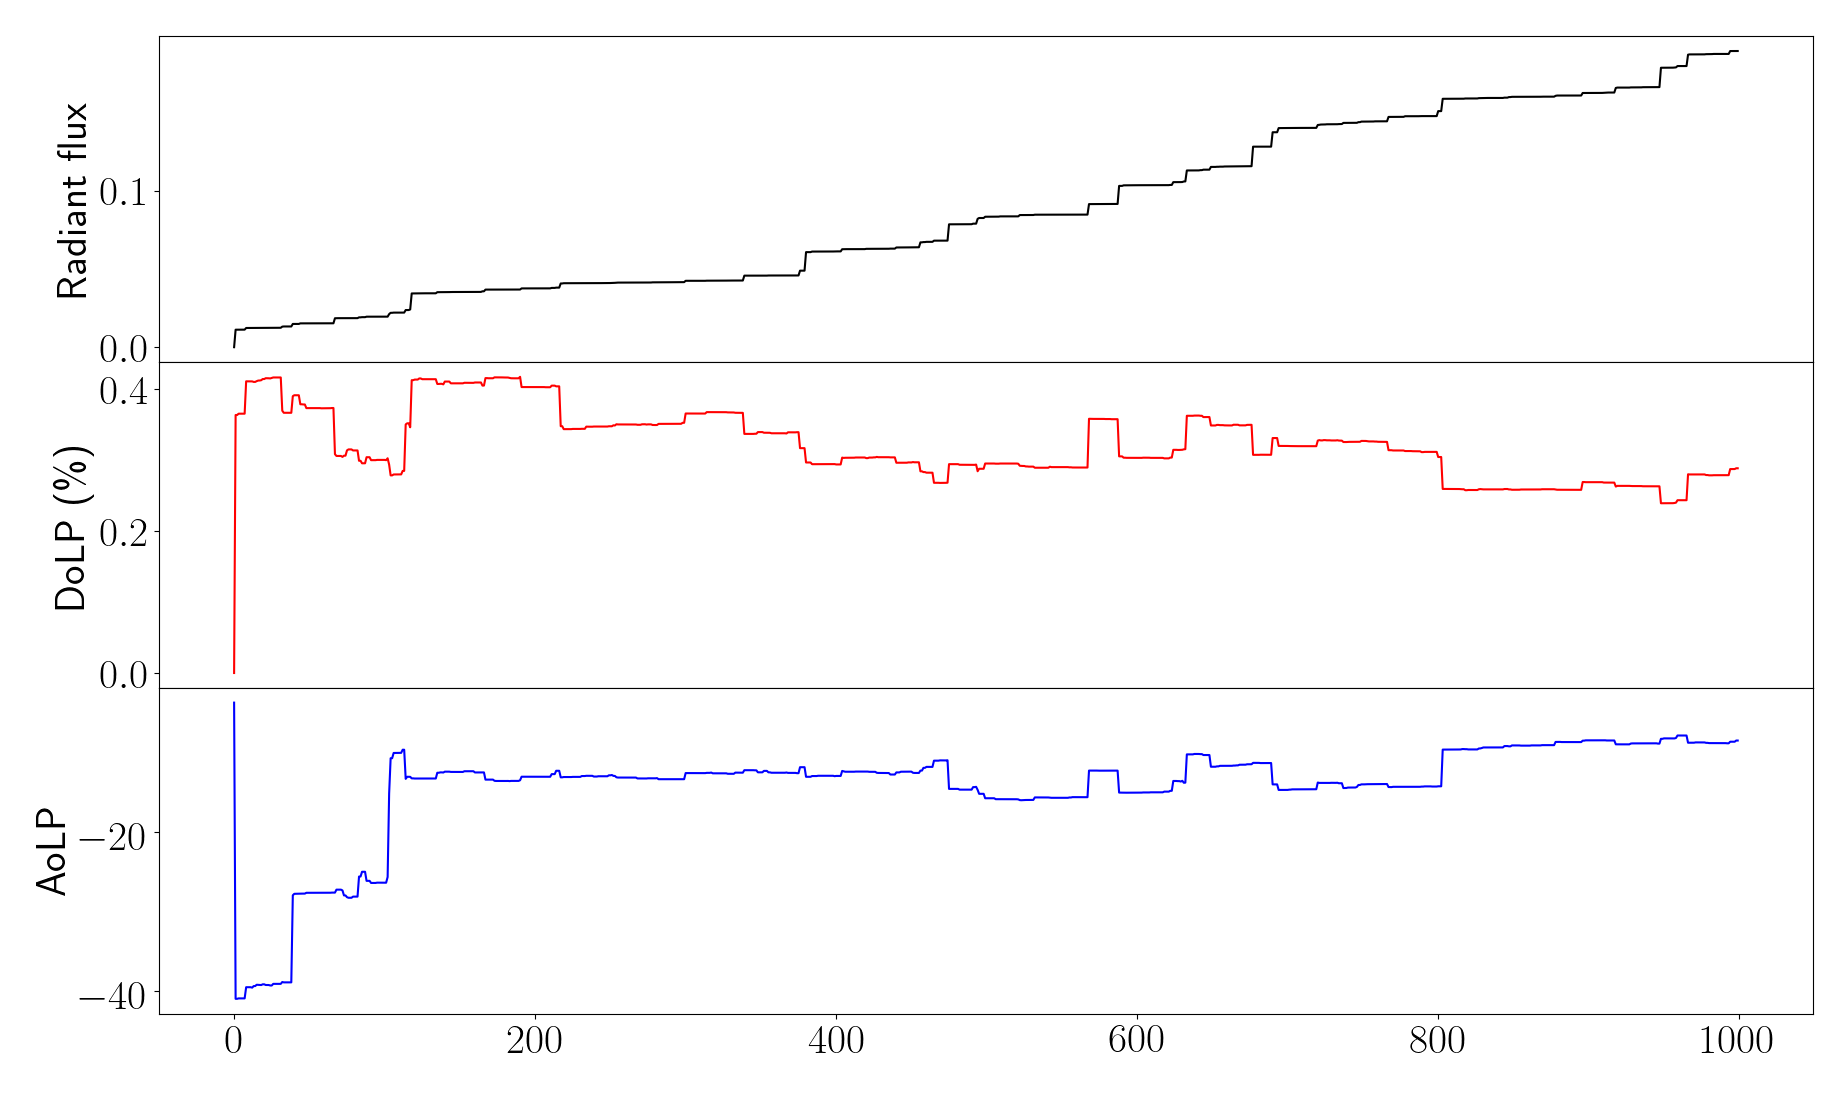
\includegraphics[width=\textwidth]{MS_cumulative_contribution.png}
  \caption{Flux, DoLP and AoLP of the total multiple scattering contribution as we add more and more rays (1000 rays in total). The instrument points at 45 degrees elevations above a unifromly emitting ground. The flux increases regularly with each additional ray. The $DoLP$ converges toward a fixed value (very close to zero). The AoLP converges as well around a fixed value (around $-10$ degrees). }
\end{figure}








\bibliography{multiple_scattering}

% \printbibliography

\end{document}
